\documentclass{article}

\title{Neural Networks and Computer Vision}
\author{Vladimir Feinberg}

\usepackage{nicefrac}
\usepackage[hidelinks]{hyperref}
\usepackage{xcolor}
\usepackage{url}
\usepackage{lmodern}
\usepackage{amsmath}
\usepackage{amsthm}
\usepackage{amssymb}
\usepackage{amsfonts}
\usepackage{enumerate}
\usepackage{graphicx}
\usepackage{fullpage}
\usepackage{bbm}
\usepackage{caption}
\usepackage{mathrsfs}
\usepackage[all]{xy}

\newcommand{\pa}[1]{ \left({#1}\right) }

\def \N {\mathbb{N}}
\def \Nbr {\mathcal{N}}
\def \Q {\mathbb{Q}}
\def \F {\mathbb{F}}
\def \then {\implies &}
\def \oif {\Longleftrightarrow &\,}
\def \given {\text{Given }&}
\def \assume {\text{Assume }&}
\def \thfr {\therefore &\enskip}
\def \bij {\leftrightarrow}
\def \inj {\rightarrowtail}
\def \sur {\twoheadedrightarrow}
\def \Z {\mathbb{Z}}
\def \R {\mathbb{R}}
\def \C {\mathbb{C}}
\def \T {\mathbb{T}}
\def \iff {\Longleftrightarrow}
\def \kron {\boldsymbol\delta}
\def \indicator {\mathbbm{1}}

\def\Ta{\textbf{a}}
\def\Tm{\textbf{m}}
\def\Tb{\textbf{b}}
\def\Tc{\textbf{c}}
\def\Td{\textbf{d}}
\def\Te{\textbf{e}}
\def\Tv{\textbf{v}}
\def\Tx{\textbf{x}}
\def\Tw{\textbf{w}}
\def\Ty{\textbf{y}}
\def\Tk{\textbf{k}}
\def\Tt{\textbf{t}}
\def\Tz{\textbf{z}}
\def\Tl{\textbf{l}}
\def\quotient{\mathclose{}/\mathopen{}}
\def\Tf{\textbf{f}}
\def\Th{\textbf{h}}
\def\Tg{\textbf{g}}
\def\sumn{\sum_{n=0}^\infty}
\def\limn{\lim_{n\rightarrow\infty}}
\def\prodn{\prod_{n=0}^\infty}

\def\bsz{\textbf{0}}
\def\bs1{\textbf{1}}
\def\bsa{{\boldsymbol\alpha}}
\def\bse{{\boldsymbol\eta}}
\def \bss{ {\boldsymbol\sigma}}
\def \bsth{ {\boldsymbol\theta}}

\DeclareMathOperator{\conv}{conv}
\DeclareMathOperator\cat{cat}
\DeclareMathOperator\adj{adj}
\DeclareMathOperator{\Laplace}{Laplace}
\DeclareMathOperator\Poisson{Poisson}
\DeclareMathOperator\Id{Id}
\DeclareMathOperator\Uniform{Uniform}
\DeclareMathOperator\mathProb{\mathbb{P}}
\def\P{\mathProb} % need to overwrite stupid paragraph symbol
\DeclareMathOperator\mathExp{\mathbb{E}}
\def \E {\mathExp}


\newcommand{\stc}[1]{\widetilde{#1}}   
\newcommand{\set}[2]{ \left\{ #1 \,\middle|\, #2 \right\} }
\newcommand{\idx}[3]{ \left\{ #1 \right\}_{ #2 }^{ #3 } }
\newcommand{\card}[1]{\left\vert{#1}\right\vert}
\newcommand{\colv}[1]{\begin{pmatrix} #1 \end{pmatrix}}
\newcommand{\mat}[1]{\begin{pmatrix} #1 \end{pmatrix}}
\newcommand{\detmat}[1]{\begin{vmatrix} #1 \end{vmatrix}}
\newcommand{\spanb}[1]{\text{span}\{ #1 \}}
\newcommand{\abs}[1]{\left|#1\right|}
\newcommand{\opcat}[1]{#1^{\text{op}}}
\newcommand{\Inner}[1]{\left\langle #1 \right\rangle}
\newcommand{\Innercpy}[1]{\Inner{ #1, #1 }}
\newcommand{\norm}[1]{\left\| #1 \right\|}% use instead of $\|x\|$

\def\eqd{\mathrel{\overset{\Delta}{=}}}

\DeclareMathOperator{\diag}{diag}
\DeclareMathOperator{\vcdim}{VC-dim}
\DeclareMathOperator*{\Err}{\text{err}}
\DeclareMathOperator*{\ErrE}{\mathbb{E}}
\DeclareMathOperator{\Tr}{tr}
\DeclareMathOperator{\Dim}{dim}
\DeclareMathOperator{\Rank}{rank}
\DeclareMathOperator*{\argmin}{argmin}
\DeclareMathOperator*{\proj}{proj}
\DeclareMathOperator{\Ker}{ker}
\DeclareMathOperator{\Diam}{diam}
\DeclareMathOperator{\Int}{int}
\DeclareMathOperator{\Clo}{clo}
\DeclareMathOperator{\sgn}{sgn}
\DeclareMathOperator{\MyRe}{Re}
\DeclareMathOperator{\MyIm}{Im}
\DeclareMathOperator{\image}{image}
\DeclareMathOperator{\colim}{colim}
\DeclareMathOperator{\Supp}{supp}
\DeclareMathOperator{\Var}{var}
\DeclareMathOperator{\Hom}{hom}
\DeclareMathOperator{\Ob}{ob}
\DeclareMathOperator{\El}{el}
\DeclareMathOperator\power{{\mathcal{P}}}
\DeclareMathOperator{\Nat}{Nat}
\DeclareMathOperator{\cone}{cone}
\DeclareMathOperator{\vectorize}{vec}
\DeclareMathOperator{\matricize}{mat}

% probability stuff
\def \sa {{$\sigma$-algebra}}
\def\OR{{\overline{\R}}}
\def\OX{{\overline{X}}}

\def\mcU{{\mathcal{U}}}
\def \mcX {\mathcal{X}}
\def \mcS {\mathcal{S}}
\def \mcY {\mathcal{Y}}
\def \mcH {\mathcal{H}}
\def \mcD {\mathcal{D}}
\def \mcC {\mathcal{C}}
\def \mcA {\mathcal{A}}
\def \mcK {\mathcal{K}}
\def \mcM {\mathcal{M}}
\def\mcG{{\mathcal{G}}}
\def\mcH{{\mathcal{H}}}
\def\mcF{{\mathcal{F}}}
\def\mcB{{\mathcal{B}}}
\def\mcE{{\mathcal{E}}}
\def\mcI{{\mathcal{I}}}
\def\mcQ{{\mathcal{Q}}}
\def\mcM{{\mathcal{M}}}
\def\mcC{{\mathcal{C}}}
\def\mcT{{\mathcal{T}}}
\def\mcO{{\mathcal{O}}}
\def\mcJ{{\mathcal{J}}}

\makeatletter
\DeclareFontFamily{U}  {MnSymbolF}{}
\DeclareSymbolFont{symbolsMN}{U}{MnSymbolF}{m}{n}
\SetSymbolFont{symbolsMN}{bold}{U}{MnSymbolF}{b}{n}
\DeclareFontShape{U}{MnSymbolF}{m}{n}{
    <-6>  MnSymbolF5
   <6-7>  MnSymbolF6
   <7-8>  MnSymbolF7
   <8-9>  MnSymbolF8
   <9-10> MnSymbolF9
  <10-12> MnSymbolF10
  <12->   MnSymbolF12}{}
\DeclareFontShape{U}{MnSymbolF}{b}{n}{
    <-6>  MnSymbolF-Bold5
   <6-7>  MnSymbolF-Bold6
   <7-8>  MnSymbolF-Bold7
   <8-9>  MnSymbolF-Bold8
   <9-10> MnSymbolF-Bold9
  <10-12> MnSymbolF-Bold10
  <12->   MnSymbolF-Bold12}{}
\DeclareMathSymbol{\tbigtimes}{\mathop}{symbolsMN}{2}
\newcommand*{\bigtimes}{%
  \DOTSB
  \tbigtimes
  \slimits@ 
}
\makeatother

% category theory arguments
% more equality: http://tex.stackexchange.com/questions/333629/
\newcommand\superequiv{ \mathrel{\rlap{\raisebox{\fontdimen22\textfont2}{$ = $}}\raisebox{-0.5\fontdimen22\textfont2}{$ = $}}}
\newcommand{\catfst}{{-}}
\newcommand{\catsnd}{{=}}
\newcommand{\cattrd}{{\equiv}}
\newcommand{\catfth}{{\superequiv}}


\newcommand{\nurl}[2]{\href{ #1 }{\color{blue}\underline{#2}}}
\usepackage{animate}

\begin{document}

\maketitle

We review techniques for computer vision with DNNs. Content is mostly from Dr. Goodfellow's \nurl{http://www.deeplearningbook.org/contents/convnets.html}{Deep Learning Book}, but also taken from \nurl{https://www.coursera.org/learn/neural-networks}{Dr. Hinton's Coursera Class}, lecture week 5.

DNN vision techniques rely critically on convolutional neural nets (CNNs). Note that the techniques here can generally be applied to other inputs with grid topology, possibly of 1 dimension (like time series: joint angle data for a robot or audio data) or more than two (such as 3D fMRI imaging). Multiple channels (such as colors, or later feature maps) can just be viewed as separate image maps or new dimensions in the data.

\section{Visual Difficulties}

Visual difficulties we'd like to avoid include segmentation (teasing apart an object from its background and other object), deformation, lighting, and viewpoint.

\section{Convolution}

Convolution is a linear operation that replaces a fully-connected layer in a neural network. Thus, whereas a fully-connected layer with a vector input $\vx$ and activation $f$ may look like $f(W\vx+\vb)$ for weight $W$ and bias $\vb$, a convolutional layer would behave like $f(\vw *\vx)$. In this context, the weight $\vw$ is referred to as a kernel, and $f$ is typically a rectifier followed by a pooling operation. It is common for multiple kernels to be applied to the same $\vx$, the pooled results of which form the output of the layer as feature maps. The terminology follows similarly when replacing the vectors $\vx,\vw$ with arbitrary tensors $\mathsf{X},\mathsf{W}$; convolutions are well-defined on them.

Convolution can be viewed as a linear operation. A 1D convolution is multiplication by a circulant matrix, a 2D convolution is multiplication by a doubly-circulant block matrix, and so on (\nurl{https://dsp.stackexchange.com/questions/35373/convolution-as-a-doubly-block-circulant-matrix-operating-on-a-vector}{example derivation}). Thus, indeed convolution is a form of parameter sharing and sparse interactions. Convolutions are typically implemented as cross-correlations. Even though this loses the commutativity property, these networks are just as expressive since we can just transpose the kernel. For small kernel sizes, convolution can be implemented much more efficiently than with their associated matrix multiplies.

Modifications or common enhancements to convolution (see \nurl{https://arxiv.org/abs/1603.07285}{Dumoulin and Visin 2016}, Fig.~\ref{fig:conv}):
\begin{itemize}
\item Padding. Various paddings add zeros around the inputs and result in different output sizes. These dictate the role that partially applied filters at the boundary will play.
\item Strides. A stride of greater than one skips applications of the kernel filter, which can be viewed as a form of regularization through downsampling. Along a similar vein, diluted convolutions apply the kernel itself at strides along the input. A transposed form of convolution, deconvolution, reverses this process, upsampling compressed input (\nurl{http://www.matthewzeiler.com/pubs/cvpr2010/cvpr2010.pdf}{Zeiler 2010}).
\item Detectors. These are the nonlinearities applied after our linear convolutional transform.
\item Degrees of parameter sharing. Unshared convolutions learn a new kernel for each application of the kernel to an input feature map, these have no sharing and are called locally connected layers. Tiled convolutions rotate through a small set of kernels as a middle ground proposed by \nurl{https://papers.nips.cc/paper/4136-tiled-convolutional-neural-networks}{Ngiam et al 2010}, but they're usually replaced by having many parallel regular convolutional layers now.
\end{itemize}


\begin{figure}[!h]
\centering
\animategraphics[autoplay,loop,width=0.5\textwidth]{1}{padding-movie/theano-pad-}{0}{35}
\caption{Demonstration of a convolutional layer with padding, no strides, and no dilation retrieved from \nurl{http://deeplearning.net/software/theano/tutorial/conv_arithmetic.html}{Theano docs}.}
\label{fig:conv}
\end{figure}

\begin{center}

\end{center}

\section{Pooling}

Pooling is typically applied after a convolutional layer/stage. It may be a nonlinear operation which is applied to a local neighborhood of the input, like a convolution. For various types of pooling and when to use them, see \nurl{http://www.di.ens.fr/willow/pdfs/icml2010b.pdf}{Boureau et al 2010}. Max-pools, for instance, encourage invariance between adjacent kernel outputs, since only one of them needs to be activated to activate the associated max pool.

Pools have a specified pool width (determining the size of the neighborhood that is pooled) and stride, which has the same effect as kernel stride.

Pooling typically reduces image width, so in cases where we would like to classify input pixels themselves, one solution is to simply produce an output at a lower resolution than the input (Fig.~\ref{fig:pinheiro}).

\begin{figure}[!h]
\centering
{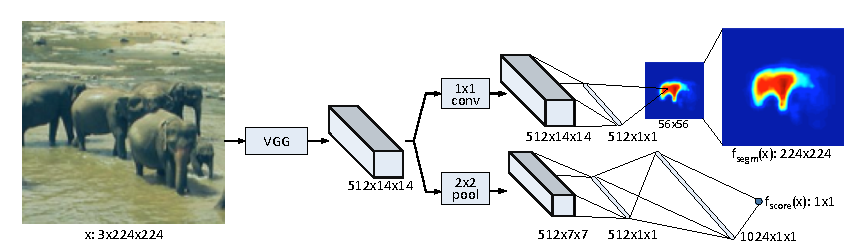
\includegraphics[width=\textwidth]{pinheiro.pdf}}
\caption{Architecture of segmentation architecture from Fig.~1 of \nurl{https://arxiv.org/abs/1506.06204}{Pinheiro et al 2015})}
\label{fig:pinheiro}
\end{figure}

Pooling isn't always necessary (\nurl{https://arxiv.org/abs/1412.6806}{Springenberg et al 2014}), and maxout-like cross-channel pooling is an interesting response (\nurl{https://arxiv.org/abs/1510.00921}{Liu et al 2015}).

\section{Initialization}

Random kernel initialization is surprisingly good, so much so that \nurl{https://cs.stanford.edu/~acoates/papers/coatesleeng_aistats_2011.pdf}{Coates et al 2011} even states that a network trained only on the last layer can be used as a selection method for CNN architectures.

\nurl{http://www.robotics.stanford.edu/~ang/papers/nipsdlufl10-RandomWeights.pdf}{Saxe et al 2010} explores unsupervised initialization approaches.

\section{Common Architectural Families}

These change very frequently and it's more useful to just study common families of networks. See this \nurl{https://adeshpande3.github.io/adeshpande3.github.io/The-9-Deep-Learning-Papers-You-Need-To-Know-About.html}{overview post}. Missing from that post but selected as important by Dr. Goodfellow is the \nurl{https://www.ncbi.nlm.nih.gov/pubmed/12201451}{spatial transducer network}.

\section{Preprocessing}

\begin{itemize}
\item Normalize data input channels from integer pixel values $[0,255]$ to floats on $[0,1]$.
\item Train on many cropped versions of the data and have classifiers vote (can this be re-interpreted as parallel CNNs, and if so how does sharing affect this technique?)
\item Denoise with respect to some cannoncial form of the data (rotations, skew). This can enable smaller models but some caution should be used. It is sometimes better to let the models figure out the cannonical form for themselves.
\item Global contrast normalization (GCN) standardizes pixel inputs; local contrast normalization (LCN) scopes deviation to a window (helps make edges stand out). GCN reduces pressure on the model to handle different scales of input intensity.
\item Random perturbations to input such as color changes or translations or rotations can help augment the dataset for better generalization (\nurl{http://yann.lecun.com/exdb/publis/pdf/lecun-98.pdf}{LeCun et al 1998b}, \nurl{https://papers.nips.cc/paper/4824-imagenet-classification-with-deep-convolutional-neural-networks}{Krizhevsky et al 2012})
\end{itemize}

\end{document}
% LocalWords: Dumoulin Visin Boureau Ngiam autoplay Theano